\paragraph{Задание 1}

Изначальная выборка:

596.33 383.19 647.44 477.37 792.69 482.05 400.08
381.28 313.42 900.00 463.59 488.34 471.48 475.06
414.22 321.03 534.87 667.84 472.06 593.00 583.34
454.50 397.68 553.65 684.05 796.19 715.45 688.49
324.96 661.44 559.07 698.96 382.79 568.19 627.06
552.12 338.17 243.64 599.94 548.57 532.31 209.61
611.21 320.79 717.78 567.37 403.42 705.66 624.11
471.04 354.48 429.41 388.35 670.01 438.85 621.10
611.86 662.92 362.38 358.76 398.89 273.35 469.37
434.85 494.38 188.17 477.30 216.81 190.81 408.04
9.00 240.83 585.51 705.23 564.10 558.02 400.77
428.32 405.27 221.73 496.03 372.93 428.31 457.70
518.59 508.23 342.10 314.49 417.41 461.55 517.25
584.51 435.63 484.29 808.20 506.08 359.76 489.47
235.19 393.88 542.45 656.96 518.78 537.45 465.59
551.23 329.04 127.73 498.11 469.92 268.03 74.54
491.10 289.69 354.53 533.77 552.07 231.61 517.18
435.38 59.80 225.38 468.84 528.83 161.00 259.54
151.32 260.25 544.46 374.75 317.44 374.20 595.16
516.74 290.70 455.10 392.82 532.09 269.01 324.98
552.81 414.07 388.27 632.44 670.02 249.29 642.66
641.95 318.12 482.56 532.18 489.71 445.34 224.29
594.73 425.48 437.70 185.61 543.90 455.33

\[h = \frac{x_{\max} - x_{\min}}{1 + 3.322\cdot\ln{n}} = 48.889\]

\begin{table}[h]
    \begin{center}
        \begin{tabular}{|l|l|l|l|l|l|l|}
            \hline
            \multicolumn{2}{|c|}{$[x_{i}..x_{i+1}]$} & $n_{i}$ & $W_{i}$ & $W_{i}/h_{i}$ & $F{}'(x)$
            & $x_{i}$
            \\
            \hline
            9       & 58.889  & 1  & 0.006 & 0.020 & 0.006 & 33.945  \\
            \hline
            58.889  & 108.778 & 2  & 0.013 & 0.040 & 0.019 & 83.834  \\
            \hline
            108.778 & 158.667 & 2  & 0.013 & 0.040 & 0.031 & 133.722 \\
            \hline
            158.667 & 208.556 & 4  & 0.025 & 0.080 & 0.056 & 183.612 \\
            \hline
            208.556 & 258.445 & 10 & 0.062 & 0.200 & 0.119 & 233.500 \\
            \hline
            258.445 & 308.334 & 7  & 0.044 & 0.140 & 0.162 & 283.389 \\
            \hline
            308.334 & 358.223 & 13 & 0.081 & 0.261 & 0.244 & 333.279 \\
            \hline
            358.223 & 408.112 & 20 & 0.125 & 0.401 & 0.369 & 383.168 \\
            \hline
            408.112 & 458.001 & 17 & 0.106 & 0.341 & 0.475 & 433.057 \\
            \hline
            458.001 & 507.890 & 23 & 0.144 & 0.461 & 0.619 & 482.946 \\
            \hline
            507.890 & 557.779 & 22 & 0.138 & 0.441 & 0.756 & 532.835 \\
            \hline
            557.779 & 607.668 & 13 & 0.081 & 0.261 & 0.837 & 582.724 \\
            \hline
            607.668 & 657.557 & 10 & 0.062 & 0.200 & 0.900 & 632.612 \\
            \hline
            657.557 & 707.446 & 10 & 0.062 & 0.200 & 0.962 & 682.502 \\
            \hline
            707.446 & 757.335 & 2  & 0.013 & 0.040 & 0.975 & 732.390 \\
            \hline
            757.335 & 807.224 & 2  & 0.013 & 0.040 & 0.987 & 782.280 \\
            \hline
            807.224 & 857.113 & 1  & 0.006 & 0.020 & 0.994 & 832.168 \\
            \hline
            857.113 & 907.002 & 1  & 0.006 & 0.020 & 1.000 & 882.058 \\
            \hline
        \end{tabular}
    \end{center}
\end{table}

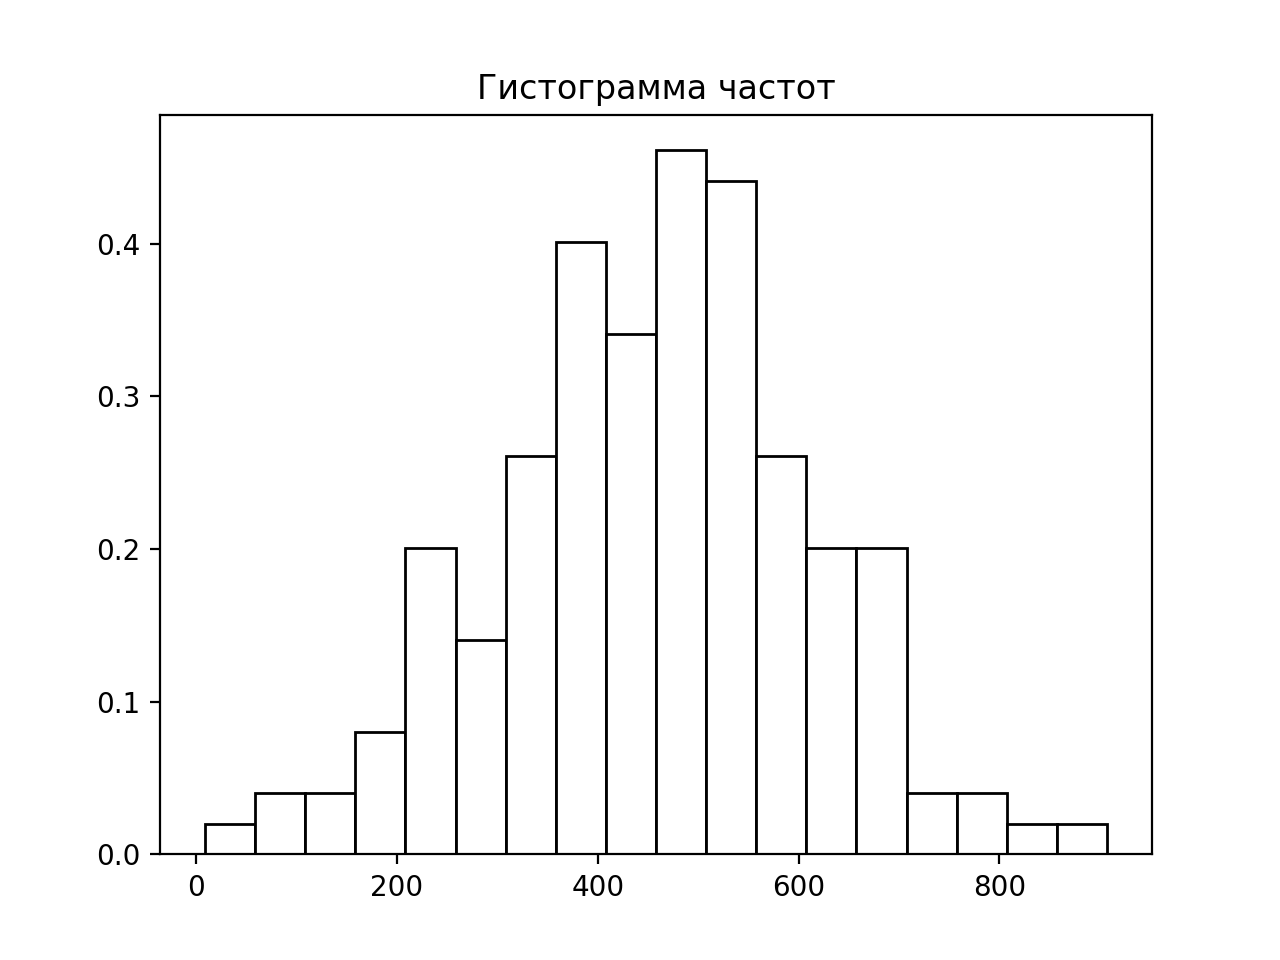
\includegraphics[width=0.9\textwidth]{src/gr11}

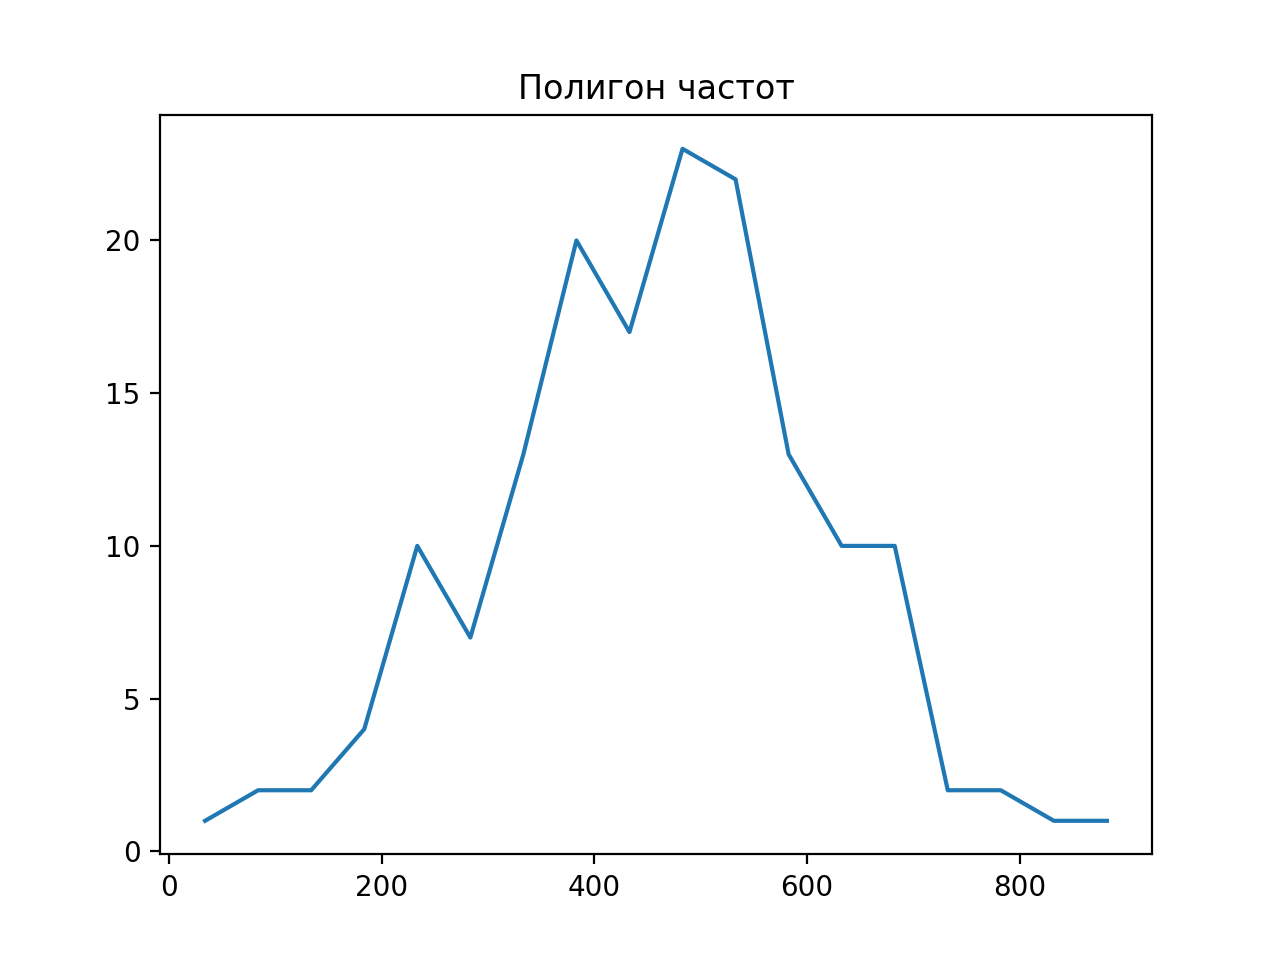
\includegraphics[width=0.9\textwidth]{src/gr12}

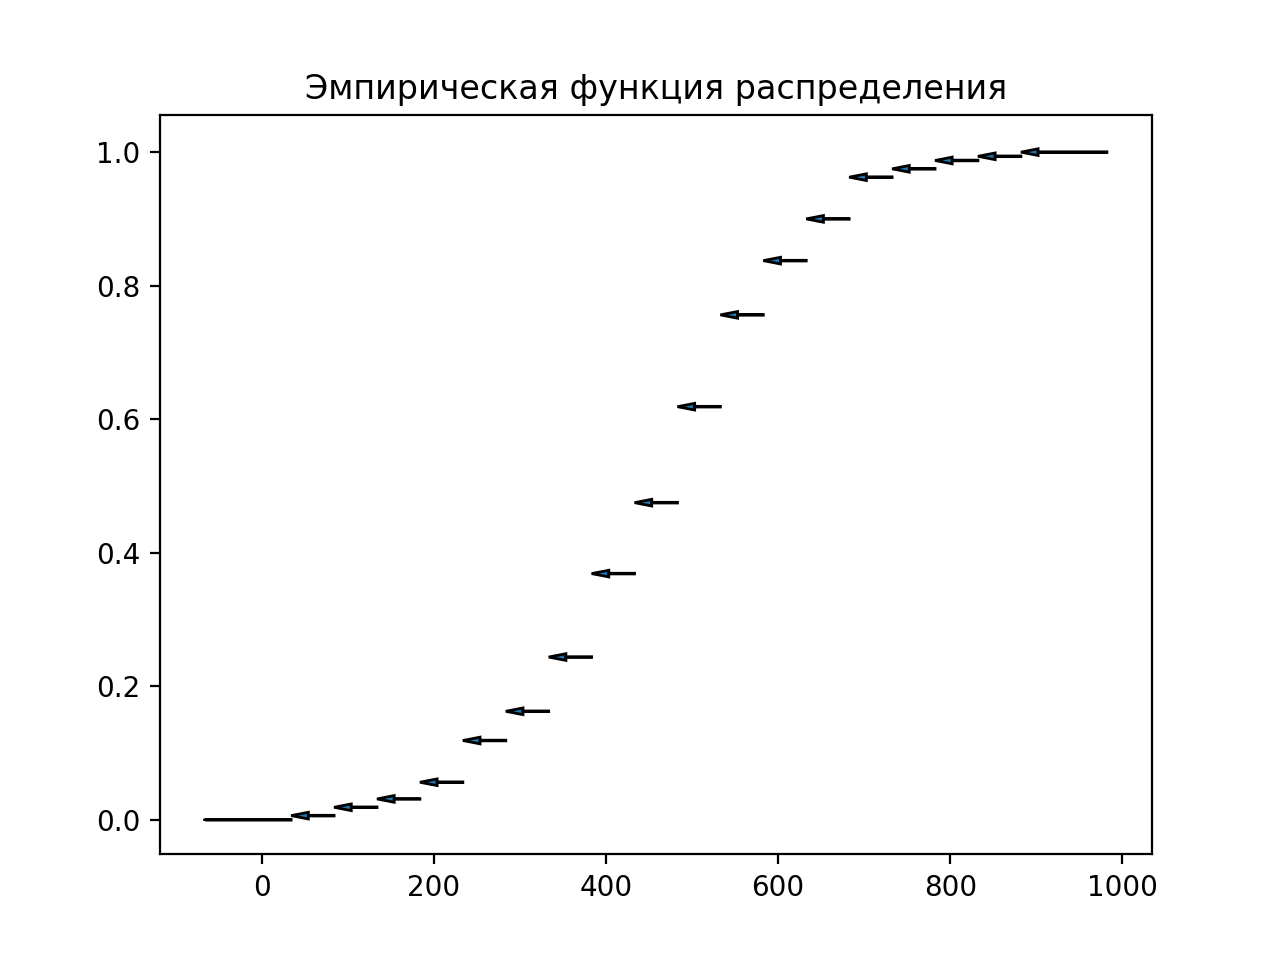
\includegraphics[width=0.9\textwidth]{src/gr13}

\begin{gather*}
    \bar{x_{s}} = 457.3773\\
    \bar{D_{s}} = 24017.6150\\
    \sigma = 154.9761\\
    S^2 = 24168.6691\\
    S = 155.4627\\
\end{gather*}